\documentclass[11pt,a4paper]{article}
\usepackage[margin=1in]{geometry}
\usepackage{amsmath,amssymb,amsthm}
\usepackage{xcolor}
\usepackage{booktabs}
\usepackage{longtable}
\usepackage{enumitem}
\IfFileExists{titlesec.sty}{%
  \usepackage{titlesec}%
  \titleformat{\section}{\large\bfseries\color{harborblue}}{\thesection}{0.7em}{}%
  \titleformat{\subsection}{\normalsize\bfseries}{\thesubsection}{0.6em}{}%
}{}
\usepackage[colorlinks=true,linkcolor=blue!45!black,urlcolor=blue!45!black]{hyperref}
\usepackage{tikz}
\IfFileExists{pgfplots.sty}{%
  \usepackage{pgfplots}%
  \pgfplotsset{compat=1.18}%
}{}
\usetikzlibrary{arrows.meta,positioning,fit,backgrounds,calc,shapes.geometric,shapes.symbols,decorations.pathmorphing,decorations.pathreplacing}
\definecolor{harborblue}{RGB}{30,70,110}
\definecolor{shipred}{RGB}{140,30,30}
\definecolor{seagreen}{RGB}{31,110,70}
\definecolor{slate}{RGB}{71,85,105}
\definecolor{slatedark}{RGB}{30,41,59}
\definecolor{amber}{RGB}{217,119,6}
\definecolor{emerald}{RGB}{16,185,129}
\newtheorem{theorem}{Theorem}
\newtheorem{claim}{Claim}
\theoremstyle{definition}
\newtheorem{change}{Change}
\newtheorem{move}{Move}
\theoremstyle{remark}
\newtheorem*{verdict}{Verdict}
\newtheorem*{adj}{Adjudication}
\setlist{itemsep=1pt,topsep=2pt}

% Shared native-figure styles for the harbor-research corpus (relation-maps,
% regime diagrams, and data plots). Vector TikZ/pgfplots only -- see
% docs/harbor-research/figures/CONVENTION.md for the house rule this follows.
\tikzset{
  relnode/.style={draw,rounded corners,thick,minimum width=2.6cm,minimum height=0.9cm,align=center,font=\small},
  relarrow/.style={-{Stealth[length=2.5mm]},thick},
  regimebox/.style={draw,thick,align=center,font=\small,inner sep=4pt},
}
\IfFileExists{pgfplots.sty}{%
\pgfplotsset{
  harbor curve/.style={
    width=0.46\textwidth,height=5.6cm,
    axis lines=left,
    label style={font=\scriptsize},
    tick label style={font=\scriptsize},
    title style={font=\small,align=center,yshift=2pt},
    legend style={font=\scriptsize,draw=black!25,fill=white,fill opacity=0.92,text opacity=1,rounded corners=1pt,inner sep=3pt},
    thick,
  },
  harbor bar/.style={
    width=0.46\textwidth,height=5.6cm,
    ybar,bar width=6pt,
    ymode=log,log origin=infty,
    axis lines=left,
    label style={font=\scriptsize},
    tick label style={font=\tiny},
    xticklabel style={rotate=40,anchor=east,font=\tiny,inner sep=1pt},
    title style={font=\small,align=center,yshift=2pt},
    legend style={font=\scriptsize,draw=black!25,fill=white,fill opacity=0.92,text opacity=1,rounded corners=1pt,inner sep=3pt},
  },
}
}{}

\usepackage{mdframed}
\usepackage{graphicx}
\graphicspath{{../figures/}}
\newmdenv[backgroundcolor=blue!4,linecolor=harborblue,linewidth=0.8pt,skipabove=6pt,skipbelow=6pt]{thebox}
\newmdenv[backgroundcolor=red!4,linecolor=shipred,linewidth=0.8pt,skipabove=6pt,skipbelow=6pt]{boundary}
\newcommand{\onebreath}[1]{\begin{center}\emph{#1}\end{center}}

\title{\textbf{Regimented or Enforced}\\[4pt]
\large The Controllability Boundary for Agent Governance\\[3pt]
\normalsize Paper 2 of the Harbor program: a supervisory-control characterization\\ of what an
agent runtime can prevent}
\author{Prepared for Erich Owens}
\date{August 2026}
\begin{document}
\maketitle

\begin{abstract}
\noindent An agent hypervisor --- a runtime that mediates an LLM agent's file writes, network
egress, tool executions, pushes, and spawns --- is asked to \emph{enforce} governance policies.
Some it can enforce by prevention: the forbidden thing never happens. Others it can only enforce
by detection and compensation: the thing happens, and the runtime notices afterward. We show the
boundary between the two is not an engineering contingency but a theorem: a prefix-closed safety
policy is \emph{regimentable} (preventable pre-effect) if and only if it is controllable in the
sense of Ramadge--Wonham supervisory control theory, with respect to the uncontrollable event
set of an LLM (model-internal steps and in-context reads). Schneider's classical result ---
execution monitors enforce exactly safety properties --- is the ambient case of this
characterization; controllability is the refinement forced by an alphabet the monitor only
partly mediates. The characterization is executable: a product-automaton checker classifies a
realistic policy set (egress, push, write, exec, spawn: regimentable; token emission, context
reads, internal plans, confident falsehoods: detect-only forever), and settles the decisive
compound case --- ``no egress after reading a secret'' \emph{is} regimentable, because the
policy permits the uncontrollable trigger and gates only the controllable effect. That single
classification is the design theorem behind clean-room agent computation: gate the channel,
never the token.
\end{abstract}

\vspace{0.5em}
\noindent\textbf{Express lane.} \emph{A governance policy can be enforced by prevention iff no
legal prefix of agent behavior can be pushed out of the policy by an event the runtime cannot
intercept --- Ramadge--Wonham controllability with respect to $\Sigma_u = \{$model-internal
steps, in-context reads$\}$; formal statement and proof in the box of \S\ref{sec:theorem},
machine-checked policy table in \S\ref{sec:table}.} Experts: read the box, the table, and
\S\ref{sec:compound}; the rest is scaffolding.

\section{The scene: two kinds of ``the runtime enforces it''}\label{sec:scene}
A team runs coding agents behind a single-writer daemon. Every file write, network call,
subprocess spawn, and \texttt{git push} passes through the daemon's effect boundary, where
policy is checked before the effect lands. The governance document lists rules: \emph{no
force-push to main}; \emph{no network egress from sandboxed jobs}; \emph{no writes outside the
granted scope}; and also \emph{no confident falsehoods in status reports}; \emph{never
incorporate the customer's secret into your plan}.

The operations lead asks the obvious question: which of these does the runtime \emph{guarantee},
and which does it merely \emph{watch for}? The first three feel different from the last two, and
every practitioner senses it. The force-push rule is airtight --- the daemon owns the git remote
credentials, and a push that never happens needs no forgiveness. The confident-lie rule is not
airtight and never will be: the lie is composed inside the model's forward pass, and by the time
any mediator sees tokens, the lie already exists. The practitioner's instinct is correct. This
paper proves it is not an instinct but an instance of a thirty-nine-year-old theorem, and
extracts the exact boundary.

\paragraph{The idea in one breath.}
\onebreath{Split the agent's event alphabet into what the runtime can refuse (mediated effects)
and what it cannot (model-internal steps); a safety policy is preventable iff no uncontrollable
event can carry a legal history out of the policy --- and that is precisely Ramadge--Wonham
controllability.}

\paragraph{Intuition: the bouncer.} A club has one door and a bouncer. The bouncer can refuse
\emph{entry} --- entry is controllable, mediated by the door. The bouncer cannot refuse a
patron's \emph{thought} --- thought is uncontrollable, unmediated by anything the club owns. A
door policy (``no entry after 2am'') is enforceable by prevention. A thought policy (``no ill
intent inside'') is enforceable only by observation and ejection --- detection and compensation.
Now the structural mapping (Figure~\ref{fig:relation}): the daemon's effect boundary is the
door; $\Sigma_c$ (fs\_write, net\_egress, exec\_tool, git\_push, spawn\_child) is entry;
$\Sigma_u$ (model\_emit\_token, in\_context\_read, internal\_plan) is thought. The analogy maps
relations, not surface features, so it earns a prediction: a \emph{compound} rule mentioning
thought but gating only the door --- ``no entry for anyone who arrived after the fight started''
--- should still be enforceable by prevention, because the bouncer needs only to \emph{observe}
the trigger and \emph{refuse} the door. Section~\ref{sec:compound} confirms exactly this for
agents.

The predictable misread, preempted: the analogy does \emph{not} say internal events are
invisible --- tokens are eminently loggable after emission. Uncontrollable means
\emph{unrefusable before the fact}, not unobservable after it. (When events are also
unobservable, a second, stricter theory applies --- \S\ref{sec:partial}.)

\begin{figure}[t]\centering
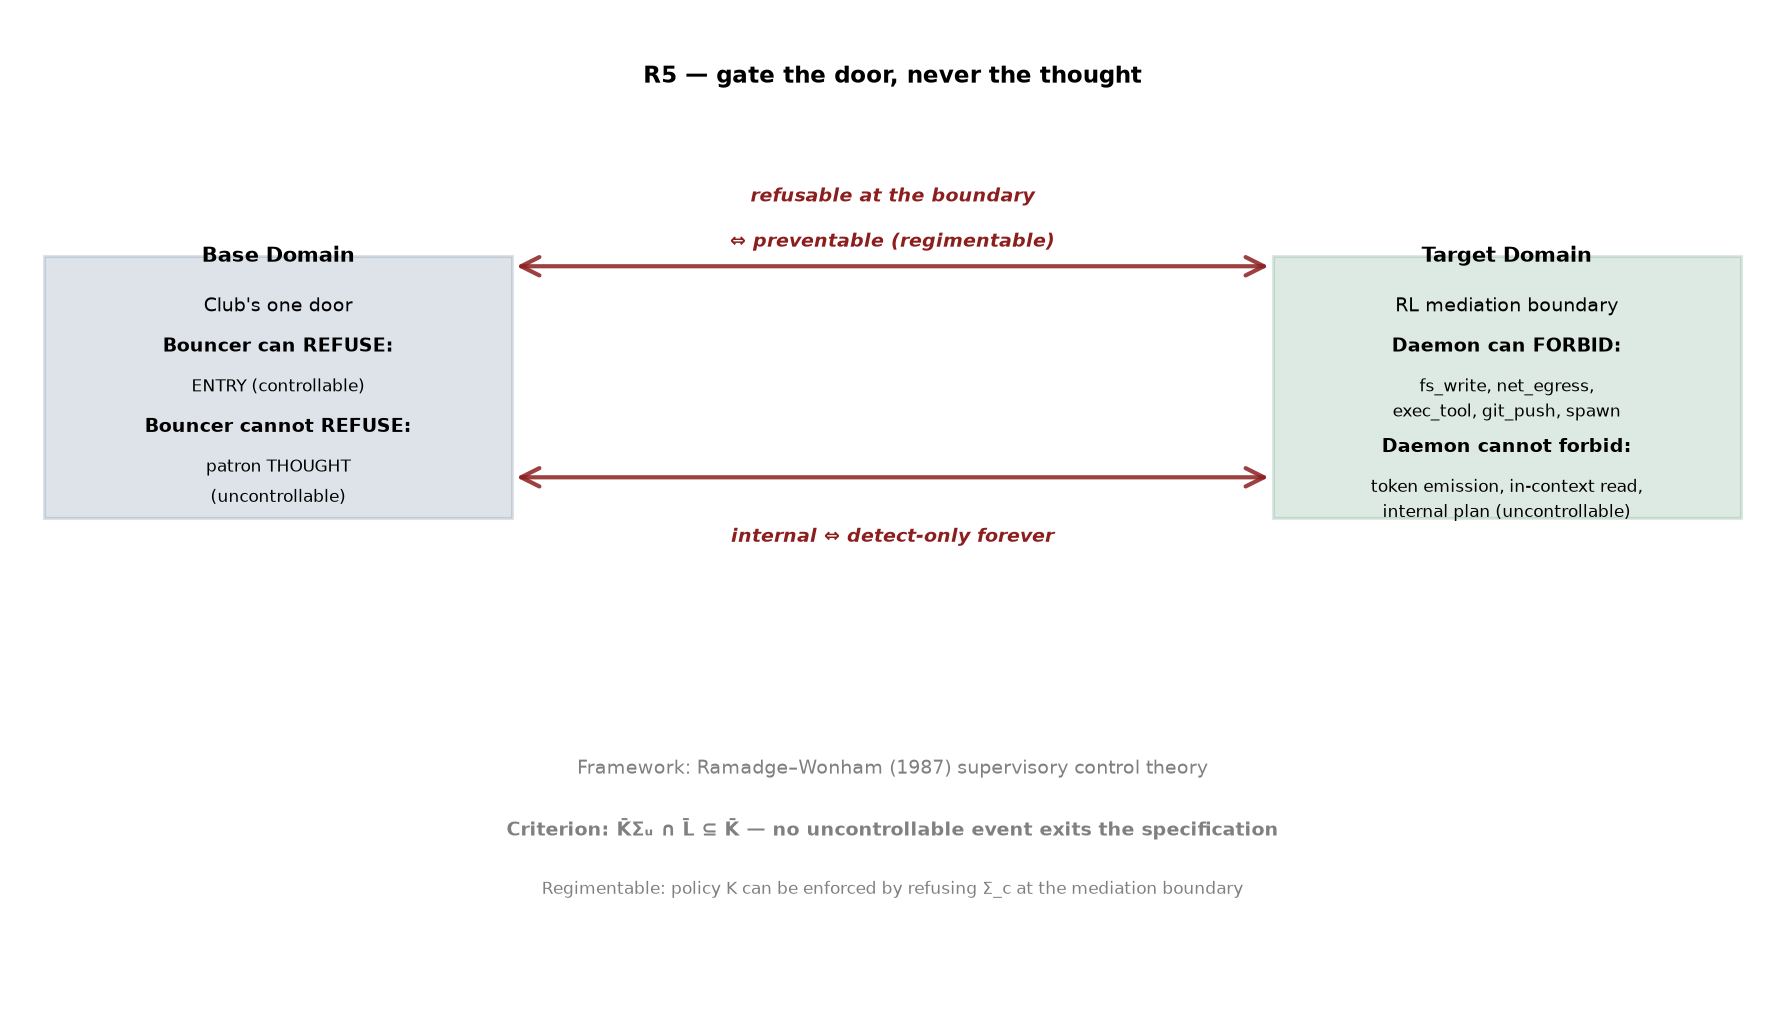
\includegraphics[width=0.92\textwidth]{r5_relation.png}
\caption{The relation map. Base domain: a club's single door --- the bouncer refuses entry
(controllable) but cannot refuse thought (uncontrollable). Target domain: the daemon's mediation
boundary --- the runtime can forbid fs\_write, net\_egress, exec\_tool, git\_push, spawn\_child,
and cannot forbid token emission, in-context reads, or internal plans. The correspondence arrows
carry the theorem: refusable-at-the-boundary $\Leftrightarrow$ preventable (regimentable);
internal $\Leftrightarrow$ detect-only forever. The criterion under the map,
$\overline{K}\Sigma_u\cap\overline{L}\subseteq\overline{K}$, is Ramadge--Wonham controllability [verified
framework].}
\label{fig:relation}
\end{figure}

\section{The model}\label{sec:model}
\paragraph{Events and the mediation boundary.} Fix a finite alphabet
$\Sigma=\Sigma_c\uplus\Sigma_u$ of agent events. $\Sigma_c$ (\emph{controllable}) contains the
events that pass through the runtime's mediation boundary before taking effect, so the runtime
can disable any of them at any instant: in our reference alphabet,
$\Sigma_c=\{$\texttt{fs\_write}, \texttt{net\_egress}, \texttt{exec\_tool}, \texttt{git\_push},
\texttt{spawn\_child}, \texttt{api\_call}$\}$. $\Sigma_u$ (\emph{uncontrollable}) contains the
events that occur before any mediator can intervene: $\Sigma_u=\{$\texttt{model\_emit\_token},
\texttt{in\_context\_read}, \texttt{internal\_plan}, \texttt{hidden\_activation}$\}$. The split
is a fact about the architecture, not a modeling choice: the daemon owns the
syscall-and-credential surface and does not own the forward pass.

\paragraph{Plant and policy.} The \emph{plant} $L\subseteq\Sigma^*$ is the prefix-closed
language of physically possible behaviors; for a general agent we take the universal plant
$L=\Sigma^*$ (any interleaving can occur). A \emph{policy} is a prefix-closed language
$K\subseteq L$: the set of allowed histories. Prefix closure makes $K$ a \emph{safety} property
in the classical sense --- a violation is witnessed by a finite prefix and can never be
un-violated. $\overline{K}$ denotes prefix closure (so $\overline{K}=K$ here; we keep the bar to
match the standard statement).

\paragraph{What ``regiment'' means.} A \emph{regimentation mechanism} is a supervisor
$f:\overline{L}\to 2^{\Sigma_c}$ mapping each history to a set of \emph{disabled controllable}
events; the supervised plant executes any event not disabled. Crucially the supervisor's type
says everything: it can disable only members of $\Sigma_c$. The mechanism \emph{regiments} $K$
if the closed-loop behavior equals $\overline{K}$ --- every allowed history remains reachable
and no violating history is reachable. Anything short of that --- allowing the violation and
then flagging, rolling back, slashing a bond --- is \emph{detect-and-compensate}, a legitimate
but categorically weaker enforcement mode.

\section{The ambient result, and why the alphabet split refines it}\label{sec:schneider}
Schneider's classical theorem says an execution monitor (EM) --- a mechanism that watches a
single execution and can terminate it --- enforces exactly the safety
properties~\cite{schneider}. That result is the \emph{ambient} case of ours: it implicitly
assumes the monitor mediates \emph{every} event, i.e.\ $\Sigma_u=\emptyset$. Under complete
mediation, controllability is vacuous (there is no uncontrollable event to carry a history out
of $K$), so ``safety'' is the entire boundary, and Schneider's theorem is exactly what our
characterization degenerates to.

An LLM agent runtime does not enjoy complete mediation. The model's forward pass emits tokens,
reads its context, and forms plans on hardware the daemon schedules but does not gate
step-by-step; these events happen and \emph{then} become visible, which in supervisory-control
terms makes them uncontrollable. Once $\Sigma_u\neq\emptyset$, safety remains \emph{necessary}
for preventability (a liveness violation has no finite witness to block) but is no longer
\emph{sufficient}: ``never \texttt{internal\_plan}'' is as prefix-closed a safety property as
``never \texttt{git\_push},'' yet only one of them is preventable. The refinement that separates
them is Ramadge--Wonham controllability~\cite{rw87,rw89}, developed for exactly this situation
--- a plant in which some events (machine breakdowns, arrivals) cannot be disabled by any
supervisor. Anderson's reference-monitor tradition~\cite{anderson} contributes the design
obligation (complete mediation \emph{of the controllable alphabet}: every $\Sigma_c$ event
actually passes the boundary), and Rushby's separation-kernel analysis~\cite{rushby} the
standard for verifying that the obligation holds; neither supplies the boundary itself. The
boundary is controllability.

\section{The theorem}\label{sec:theorem}
\begin{thebox}
\textbf{Theorem (Regimentation $=$ controllability).} Let $L\subseteq\Sigma^*$ be a
prefix-closed plant over $\Sigma=\Sigma_c\uplus\Sigma_u$, and let $K\subseteq L$ be a nonempty
prefix-closed safety policy. There exists a regimentation mechanism for $K$ --- a supervisor
disabling only controllable events whose closed loop realizes exactly $\overline{K}$ --- if and
only if $K$ is \emph{controllable} with respect to $L$ and $\Sigma_u$:
\[
\overline{K}\,\Sigma_u\;\cap\;\overline{L}\;\subseteq\;\overline{K},
\]
i.e.\ no uncontrollable event, physically enabled after a legal history, exits the policy. When
the condition fails, no runtime confined to disabling $\Sigma_c$ can prevent the violation; the
best achievable enforcement is detect-and-compensate, and the largest preventable weakening of
the policy is the supremal controllable sublanguage $\sup\mathcal{C}(K)$, which exists and is
computable for regular $K$ and $L$ [verified framework, Ramadge--Wonham 1987].
\end{thebox}

\begin{proof}
($\Leftarrow$) Suppose $K$ is controllable. Define the supervisor $f(s)=\{a\in\Sigma_c :
sa\in\overline{L}\setminus\overline{K}\}$ for $s\in\overline{K}$: after any legal history,
disable exactly the controllable events that would exit the policy. We show the closed-loop
language equals $\overline{K}$, by induction on history length. The empty history lies in
$\overline{K}$ (nonempty and prefix-closed). Assume the current history $s\in\overline{K}$. Any
event $a$ the closed loop can execute next is enabled in the plant ($sa\in\overline{L}$) and not
disabled. If $a\in\Sigma_c$, then $a\notin f(s)$ means $sa\in\overline{K}$ by construction. If
$a\in\Sigma_u$, then $sa\in\overline{K}\Sigma_u\cap\overline{L}\subseteq\overline{K}$ by
controllability. Either way the closed loop stays in $\overline{K}$, so its language is
contained in $\overline{K}$. Conversely every $sa\in\overline{K}$ is reachable: $a\in\Sigma_u$
is never disabled, and $a\in\Sigma_c$ with $sa\in\overline{K}$ is not in $f(s)$; so containment
is equality, and $f$ regiments $K$.

($\Rightarrow$) Suppose $K$ is not controllable: there exist $s\in\overline{K}$ and
$\sigma\in\Sigma_u$ with $s\sigma\in\overline{L}$ but $s\sigma\notin\overline{K}$. Let $M$ be
any regimentation mechanism for $K$. Since $M$ realizes exactly $\overline{K}$, the legal
history $s$ is reachable under $M$ --- $M$ cannot forbid it without cutting $\overline{K}$ down.
At $s$, the plant enables $\sigma$, and $M$ cannot disable it: $\sigma\notin\Sigma_c$, and
disabling it is outside $M$'s type --- physically, the event completes before the mediation
boundary sees it. So the closed loop under $M$ reaches $s\sigma\notin\overline{K}$,
contradicting the assumption that $M$'s closed loop is contained in $\overline{K}$. Hence no
regimentation mechanism exists, and any enforcement of $K$ must tolerate the reachable violation
$s\sigma$ --- observe it after the fact and respond, which is detect-and-compensate by
definition. The existence, uniqueness, and computability of $\sup\mathcal{C}(K)$ are imported
from Ramadge--Wonham~\cite{rw87}: controllable sublanguages of $K$ are closed under arbitrary
union, so a supremal element exists, and for regular languages it is computed by a fixpoint
iteration on the product automaton.
\end{proof}

Two remarks on what the proof used. First, the forward direction is constructive and
\emph{maximally permissive}: the supervisor disables nothing except the controllable exits, so
regimentation costs no legal behavior --- the governance rule and the agent's freedom are not in
tension when the rule is controllable. Second, the reverse direction used nothing about the
mechanism except its type ($f:\overline{L}\to2^{\Sigma_c}$). No cleverness inside the runtime
--- better prompts, faster monitors, a smarter policy engine --- escapes the theorem, because
the obstruction is that $\sigma$ finishes before any decision point the runtime owns.

\section{The characterization, made runnable}\label{sec:table}
The controllability test is decidable by a product-automaton search: walk the synchronous
product of plant and policy automaton; flag any reachable product state where the plant enables
an uncontrollable event that the policy disables. We implemented the test over the reference
alphabet and ran it on the governance policy set. The
checker\footnote{\texttt{skills/harbor-results/scripts/b3\_controllability.py}; deterministic,
no seed needed; exits 0.} produces:

\begin{center}
\begin{tabular}{@{}llc@{}}
\toprule
Policy & Event class & Regimentable? \\
\midrule
forbid \texttt{net\_egress} & controllable & \textbf{yes} (regiment) \\
forbid \texttt{git\_push} (incl.\ force-push) & controllable & \textbf{yes} (regiment) \\
forbid \texttt{fs\_write} (out-of-scope write) & controllable & \textbf{yes} (regiment) \\
forbid \texttt{exec\_tool} & controllable & \textbf{yes} (regiment) \\
forbid \texttt{spawn\_child} & controllable & \textbf{yes} (regiment) \\
forbid \texttt{model\_emit\_token} & uncontrollable & no (detect only) \\
forbid \texttt{in\_context\_read} & uncontrollable & no (detect only) \\
forbid \texttt{internal\_plan} (``confident lie'') & uncontrollable & no (detect only) \\
\midrule
compound: no \texttt{net\_egress} after secret \texttt{in\_context\_read} & mixed & \textbf{yes}
(regiment) \\
\bottomrule
\end{tabular}
\end{center}

\noindent All nine verdicts are the checker's output, verbatim in content [internal,
\texttt{b3\_controllability.py}]; the eight single-event rows also follow by hand from the
theorem, which is the right way to first believe the table. \emph{Numbers by hand:} take
``forbid \texttt{git\_push}.'' The policy automaton has one state with every event except
\texttt{git\_push} self-looping; \texttt{git\_push}$\;\in\Sigma_c$, so the only event the policy
ever disables is controllable, the premise of a controllability violation ($\sigma\in\Sigma_u$
enabled in plant, disabled in policy) is unsatisfiable, and $K$ is controllable ---
regimentable. Now take ``forbid \texttt{internal\_plan}'': the same one-state automaton disables
\texttt{internal\_plan}$\;\in\Sigma_u$, the universal plant enables it at the start state, so
the empty history $s=\varepsilon\in\overline{K}$ and $\sigma=$ \texttt{internal\_plan} witness
$\overline{K}\Sigma_u\cap\overline{L}\not\subseteq\overline{K}$ --- detect-only, forever, for
any runtime with this alphabet split. \emph{Now you try:} classify ``forbid \texttt{api\_call}
after \texttt{spawn\_child}'' and ``forbid \texttt{internal\_plan} after \texttt{fs\_write}.''
(Answers: the first gates a controllable event on a controllable trigger --- regimentable; the
second must disable an uncontrollable event in its post-trigger state, and the plant enables it
there --- detect-only.)

This table is the manuscript's needed re-grading of governance rules, stated correctly:
\emph{force-push, unauthorized egress, and out-of-scope writes are matters of structural
authority and shall be prevented; a confident lie in a status report is semantic,
uncontrollable, and shall be detected and compensated} --- by audit, reputation, and slashing,
which is the adjacent paper's machinery, not this one's.

\begin{figure}[t]\centering
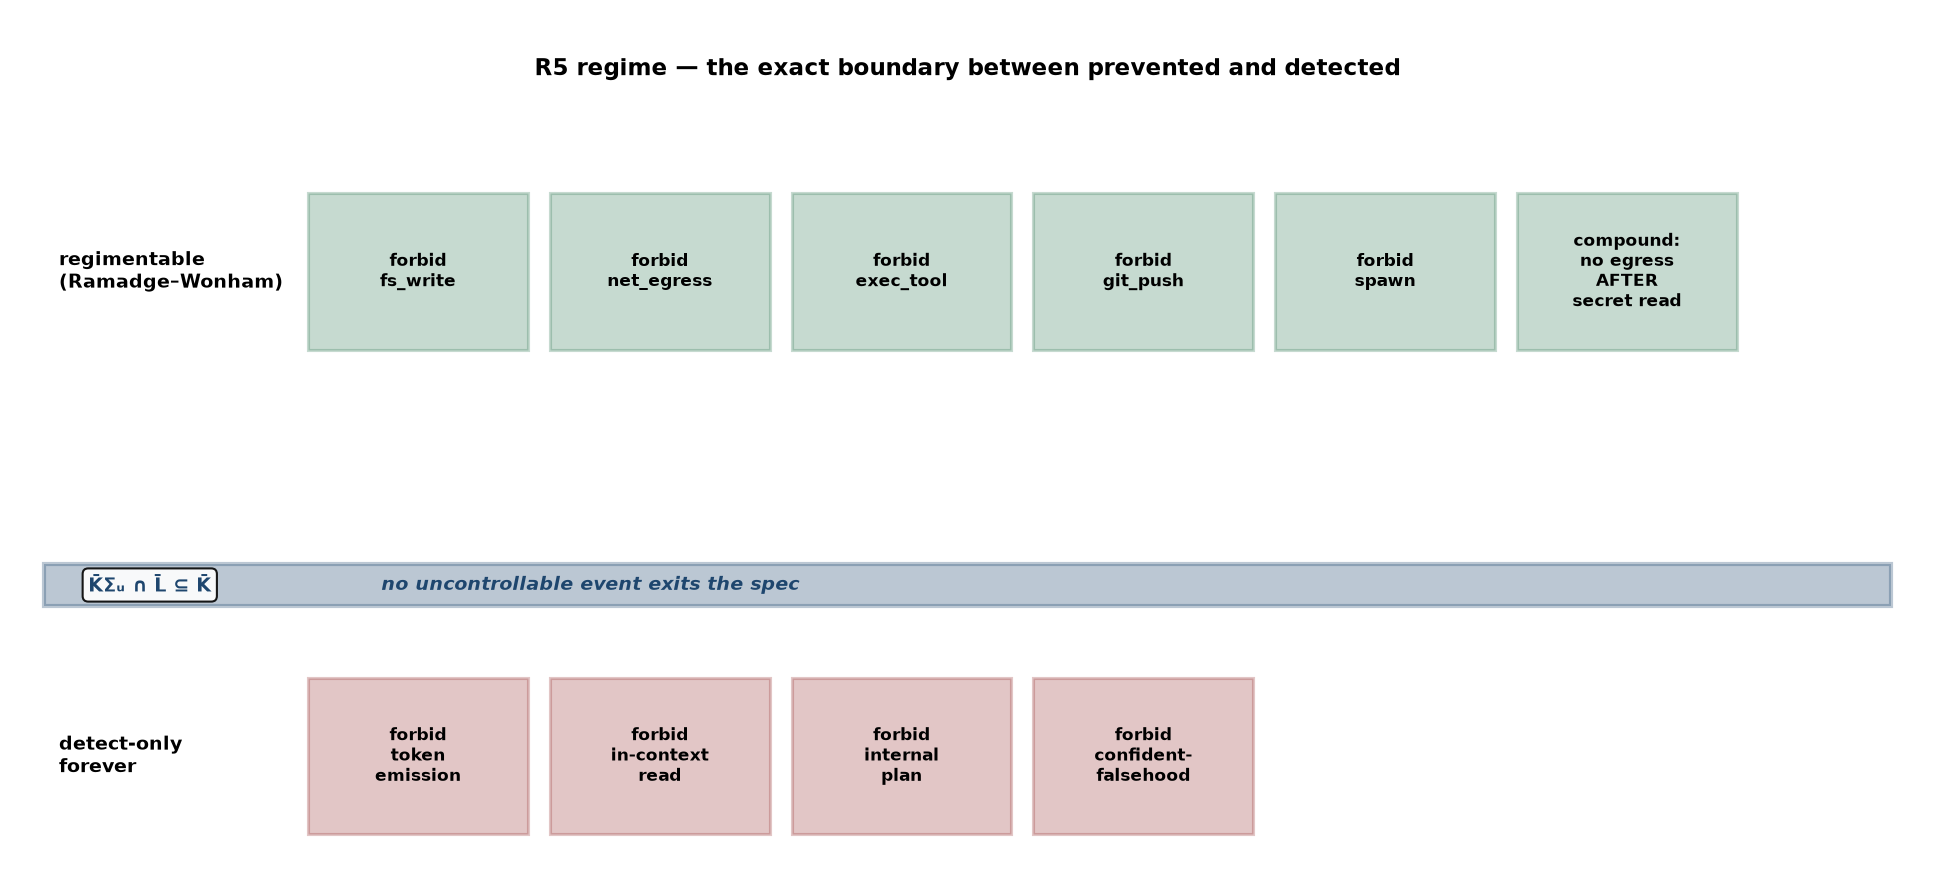
\includegraphics[width=0.95\textwidth]{r5_regime.png}
\caption{The regime diagram. Above the divider, the regimentable regime (Ramadge--Wonham
controllable): forbid fs\_write / net\_egress / exec\_tool / git\_push / spawn, and the compound
``no egress after secret read.'' Below, detect-only forever: forbid token emission / in-context
read / internal plan / confident falsehood. The divider carries the criterion
$\overline{K}\Sigma_u\cap\overline{L}\subseteq\overline{K}$ --- no uncontrollable event exits
the specification. Classifications reproduce from the product-automaton checker [internal,
\texttt{b3\_controllability.py}].}
\label{fig:regime}
\end{figure}

\section{The compound case: gate the channel, never the token}\label{sec:compound}
The last table row is the one the whole clean-room product line rests on, and it is the case
where untrained intuition most often guesses wrong. The policy \emph{``no network egress after
an in-context read of a secret''} mentions an uncontrollable event (\texttt{in\_context\_read})
--- so a naive reading of the single-event rows predicts detect-only. The checker says
otherwise:

\begin{verbatim}
COMPOUND POLICY: 'no net_egress after in_context_read of a secret'
  regimentable? YES
\end{verbatim}

\noindent [internal, \texttt{b3\_controllability.py}]. The mechanism is visible in the policy
automaton: two states, \texttt{ok} and \texttt{tainted}. The uncontrollable read is
\emph{enabled in both} --- the policy never tries to forbid it; it lets the read happen and
records the taint transition. What the tainted state disables is \texttt{net\_egress} alone, and
egress is controllable. Check the criterion: every uncontrollable event enabled by the plant is
enabled by the policy in every reachable state, so
$\overline{K}\Sigma_u\cap\overline{L}\subseteq\overline{K}$ holds and the theorem's constructive
direction hands us the supervisor --- track taint, gate the channel.

Three consequences, in increasing order of consequence.

\emph{First, the design rule.} A compound trigger$\to$effect policy is regimentable iff its
\emph{effect} events are controllable; the trigger may be as uncontrollable as it likes,
provided the policy observes rather than forbids it. Uncontrollable events in the policy's
\emph{condition} are free; uncontrollable events in its \emph{prohibition} are fatal.

\emph{Second, the clean room.} The Sealed Harbor design (Paper 4) puts an agent alone in a room
with a customer's secret data and promises the secret does not leave. The theorem dictates the
only sound architecture: it is impossible to prevent the model from \emph{reading} the secret
(the read is uncontrollable --- and useless to forbid, since reading is the job), and it is
impossible to prevent the model from \emph{incorporating} the secret into tokens and plans
(uncontrollable again). What is possible --- exactly and only --- is to gate every controllable
egress channel out of the room, with taint recorded from the moment of exposure. Gate the
channel, never the token. The companion noninterference result (R9) proves from the other
direction that the gate suffices: observations outside the room are identical across secrets
except at declared gate releases. Controllability says the gate is the only place a guarantee
\emph{can} live; noninterference says a guarantee \emph{does} live there. B3 is thus the
load-bearing assumption named in the clean-room ledger results: ``all spend is recorded'' is
precisely complete mediation of $\Sigma_c$.

\emph{Third, the special case that explains a folk theorem.} Product reviews of agent governance
converged on the slogan ``a rule is enforceable iff it is a pure deterministic function of
committed local DB state.'' That slogan is our theorem's special case $\Sigma_c=\{$DB
writes$\}$: when the only mediated channel is the database commit, the regimentable policies are
exactly those expressible over committed state. The general statement strictly dominates it ---
the slogan cannot express why force-push is preventable by a runtime that also owns the git
credential channel, nor why a confident lie stays unpreventable no matter how much state is
committed. Widening $\Sigma_c$ (owning more channels) is the \emph{only} way to grow the
regimentable set; no policy-language cleverness does.

\section{A synthesis case study: the sandboxed review job}\label{sec:synthesis}
The theorem's constructive direction is not just an existence proof --- it is the synthesis
algorithm the Supremica / TCT tool family implements, and it is small enough here to run by
hand. Consider a realistic composite policy for a sandboxed code-review job:
\begin{itemize}
\item $P_1$: no \texttt{net\_egress}, ever (sandboxed);
\item $P_2$: no \texttt{git\_push}, ever (review jobs propose, humans land);
\item $P_3$: after any \texttt{in\_context\_read} of customer material, no \texttt{fs\_write}
(findings leave through the mediated report channel, not the workspace).
\end{itemize}
Each $P_i$ is a safety automaton; the composite policy is their synchronous product. $P_1$ and
$P_2$ are one-state automata, $P_3$ is the two-state taint automaton of \S\ref{sec:compound}, so
the product spec has $1\times1\times2=2$ states, \texttt{ok} and \texttt{tainted}, and the
product with the universal one-state plant has the same two reachable states. The
controllability check visits both states and tests each of the four uncontrollable events in
each: all eight (state, event) pairs are enabled by the spec --- neither state ever disables a
member of $\Sigma_u$ --- so there are $0$ violations and the composite is controllable [verified:
eight cases, checkable by eye]. The maximally permissive supervisor falls out of the
proof's construction as a two-row disablement map:
\begin{center}
\begin{tabular}{@{}lll@{}}
\toprule
Supervisor state & Disabled ($\subseteq\Sigma_c$) & Everything else \\
\midrule
\texttt{ok} & \{\texttt{net\_egress}, \texttt{git\_push}\} & enabled \\
\texttt{tainted} & \{\texttt{net\_egress}, \texttt{git\_push}, \texttt{fs\_write}\} & enabled \\
\bottomrule
\end{tabular}
\end{center}
Two states, one observed transition (\texttt{in\_context\_read} flips \texttt{ok} to
\texttt{tainted}), three gates. That table \emph{is} the synthesized supervisor --- it is also,
not coincidentally, exactly the policy engine a competent engineer would have written by hand.
The value of synthesis is not that the answer is surprising; it is that the answer arrives with
a maximal-permissiveness certificate (no legal behavior was sacrificed) and a controllability
certificate (no uncontrollable event can force a violation), neither of which hand-written
policy engines carry.

Synthesis is equally informative when it fails. Ask it to weaken the detect-only policy ``forbid
\texttt{internal\_plan}'' to its best preventable approximation: the supremal controllable
sublanguage. Let $K'\subseteq K$ be any nonempty controllable sublanguage; it contains
$\varepsilon$, the plant enables \texttt{internal\_plan} at $\varepsilon$, so controllability
forces $\varepsilon\cdot\texttt{internal\_plan}\in\overline{K'}\subseteq\overline{K}$ ---
contradicting that $K$ forbids it. Hence $\sup\mathcal{C}(K)=\emptyset$ [verified: three lines,
above]. The theory refuses to pretend: there is no nontrivial preventable weakening of a thought
ban --- the nearest preventable policy prevents nothing --- and any governance document claiming
to ``partially enforce'' such a rule by prevention is describing detection with optimistic
vocabulary.

\section{Partial observation: the next boundary (future work)}\label{sec:partial}
Our theorem assumes the supervisor \emph{observes} every event, even the ones it cannot disable
--- the daemon logs tokens after emission, reads after completion. Realistic deployments break
this in a second place: some events are not only unrefusable but \emph{unobservable}
(activations never surfaced; state internal to a third-party tool; another principal's context).
Supervisory control under partial observation is also solved territory: Lin--Wonham~\cite{lw88}
characterize enforceability as controllability \emph{plus observability} --- the supervisor's
decisions must be constant on observation-equivalence classes of histories, i.e.\ the policy may
not demand different gate decisions after histories the runtime cannot tell apart. Observability
strictly shrinks the regimentable set: a policy like ``no egress after the model
\emph{considered} exfiltration'' references unmediated internal \emph{state} with no observable
taint transition, so even though its prohibition (egress) is controllable, no supervisor can
implement the gate condition. The practical reading: a compound policy is deployable only if its
trigger is \emph{witnessed at the mediation boundary} (the secret arrives via a mediated
\texttt{in\_context\_read} the daemon performs, as in \S\ref{sec:compound}) --- taint must be an
event the daemon sees, not a state it infers. Mapping the agent-governance policy corpus across
the observability line, and connecting it to the assurance-level ladder (which integration tiers
witness which triggers), is the natural sequel; we state it as future work rather than claim it,
because the interesting part --- which real triggers are witnessed at which assurance levels ---
is an empirical systems question, not a corollary.

\section{Related work}\label{sec:related}
Supervisory control of discrete-event systems originates with Ramadge and
Wonham~\cite{rw87,rw89}; we import controllability, the supremal controllable sublanguage, and
the maximally permissive supervisor unchanged, and claim no new control theory. Lin and
Wonham~\cite{lw88} supply the partial-observation refinement sketched in \S\ref{sec:partial}.
Schneider~\cite{schneider} characterizes EM-enforceable policies as safety properties; our
contribution relative to Schneider is the refinement under incomplete mediation
($\Sigma_u\neq\emptyset$), where safety is necessary but controllability is the exact boundary.
The reference-monitor lineage --- Anderson's complete-mediation obligation~\cite{anderson},
Rushby's kernel-verification standard~\cite{rushby}, and Goguen--Meseguer's
policy-as-noninterference framing~\cite{gm82} --- supplies the architecture our $\Sigma_c$
presumes and the companion theory Paper 4 builds on. Recent agent-guardrail work (2024--2026)
invokes this security canon for LLM runtimes but, to our knowledge from an August-2026 survey,
does not state the controllability characterization; the mapping of agent-runtime enforcement
onto supervisory control, and the resulting exact prevented/detected boundary, is the
contribution --- with the honest corollary that decades of synthesis results (supremal
sublanguages, modular and hierarchical supervision, Supremica-class tooling) now import
wholesale into agent governance. A final lit-sweep before submission is owed: ``not found'' is
not ``proven nonexistent.''

\section{Honest boundary}\label{sec:boundary}
\begin{boundary}
\textbf{What this theorem does NOT say.} (i) It does not say detect-only policies are
unenforceable or hopeless --- detection feeding audit, reputation, and bond-slashing (Paper 3)
is real enforcement; the theorem only says prevention is off the table, so pricing and
compensation must be sized for violations that \emph{will} occur. (ii) It does not certify any
implementation: the theorem's $\Sigma_c$ is the set of events \emph{actually} mediated, and
every unenumerated side channel (raw sockets, DNS, inherited file descriptors, /proc, git
credential helpers, package managers, clipboard, provider callbacks) silently moves events from
$\Sigma_c$ to $\Sigma_u$ and shrinks the regimentable set behind the operator's back ---
complete mediation of the claimed alphabet is an architectural obligation (Anderson; Rushby)
that a red-team, not this proof, discharges. (iii) The classification is relative to the
alphabet split: a runtime that gates model steps (e.g.\ token-level filtering with the model
inside the boundary) changes $\Sigma_u$ and re-grades the table --- the theorem is a functor
from architectures to boundaries, not one fixed verdict. (iv) The full-observation assumption is
load-bearing: policies whose triggers are unwitnessed internal state fall to the Lin--Wonham
refinement (\S\ref{sec:partial}) even when their prohibitions are controllable. (v) The checker
verifies the stated policy automata over the stated alphabet [internal,
\texttt{b3\_controllability.py}]; it is a faithful implementation of the test, not a mechanized
proof of the theorem --- an Isabelle/Coq formalization remains the submission gate. (vi)
Prevention governs \emph{effects}, never \emph{semantics}: no widening of $\Sigma_c$ ever makes
a confident lie preventable, because the lie is constituted, not merely caused, by
uncontrollable events.
\end{boundary}

\vspace{0.4em}
\noindent\emph{Reproducibility.} The policy table and the compound-case verdict regenerate
deterministically from \texttt{skills/harbor-results/scripts/b3\_controllability.py} (pure
Python, no dependencies, no randomness); the two figures regenerate from
\texttt{docs/harbor-research/figures/src/r5\_figures.py}. Every number and verdict in this paper
is tagged [verified] (externally recomputable from the cited literature or by hand) or [internal]
(regenerates from the named script).

\begin{thebibliography}{9}
\bibitem{rw87} P.~J. Ramadge and W.~M. Wonham. Supervisory control of a class of discrete event
processes. \emph{SIAM Journal on Control and Optimization}, 25(1):206--230, 1987.
\bibitem{rw89} P.~J. Ramadge and W.~M. Wonham. The control of discrete event systems.
\emph{Proceedings of the IEEE}, 77(1):81--98, 1989.
\bibitem{lw88} F.~Lin and W.~M. Wonham. On observability of discrete-event systems.
\emph{Information Sciences}, 44(3):173--198, 1988.
\bibitem{schneider} F.~B. Schneider. Enforceable security policies. \emph{ACM Transactions on
Information and System Security}, 3(1):30--50, 2000.
\bibitem{anderson} J.~P. Anderson. \emph{Computer Security Technology Planning Study}. Technical
Report ESD-TR-73-51, U.S. Air Force Electronic Systems Division, 1972.
\bibitem{rushby} J.~Rushby. \emph{Noninterference, Transitivity, and Channel-Control Security
Policies}. Technical Report CSL-92-02, SRI International, December 1992.
\bibitem{gm82} J.~A. Goguen and J.~Meseguer. Security policies and security models. In
\emph{Proceedings of the IEEE Symposium on Security and Privacy (Oakland)}, pages 11--20, 1982.
\end{thebibliography}
\end{document}
